\documentclass[11pt,a4paper]{article}
\usepackage[utf8]{inputenc}
\usepackage[T1]{fontenc}
\usepackage[spanish,es-nodecimaldot]{babel}
\usepackage{lmodern}
\usepackage[margin=2.3cm]{geometry}
\usepackage{graphicx}
\usepackage{booktabs}
\usepackage{amsmath}
\usepackage{float}
\usepackage{listings}
\usepackage{xcolor}
\usepackage[colorlinks=true,linkcolor=blue,urlcolor=blue]{hyperref}

\lstset{language=Python, basicstyle=\ttfamily\footnotesize, frame=single,
  keywordstyle=\color{blue!70!black}, commentstyle=\color{gray}, columns=fullflexible,
  breaklines=true, literate={á}{{\'a}}1 {é}{{\'e}}1 {í}{{\'i}}1 {ó}{{\'o}}1 {ú}{{\'u}}1 {ñ}{{\~n}}1 {ü}{{\"u}}1}
\newcommand{\code}[1]{\texttt{#1}}

\title{Laboratorio 09\\[2pt]\large Bag of Words, Similitud de Coseno e Índice Invertido}
\author{Juan Marcos Guerrero Cueva \and Adrian Urbina Mendoza \and Hector Huaman Puiquin\\[6pt]
\small Base de Datos II -- Prof. Heider Sanchez -- 2026-2}
\date{16 de octubre de 2026}

\begin{document}
\maketitle
\tableofcontents

\section{P1. Configuración y carga de datos}
Se usó PostgreSQL 17.5 y Python 3.13 (pandas, psycopg2, NLTK, Matplotlib). El notebook
\code{lab09.ipynb} crea la base y las tablas \code{noticias} y \code{stopwords} con el esquema
del enunciado, y carga \code{news\_es.csv} (1217 noticias) y \code{stoplist.txt} (608 stopwords).
Solo inserta datos si las tablas están vacías, así que se puede volver a ejecutar sin duplicar filas.
Las credenciales se leen de un archivo \code{.env}, que no se sube al repositorio.

\section{P2. Preprocesamiento y Bag of Words}
\code{preprocess} aplica cuatro pasos: minúsculas, tokenización (solo secuencias de letras, sin
números ni signos), eliminación de las stopwords leídas de la tabla y stemming Snowball para
español. \code{compute\_bow} cuenta la frecuencia de cada término y \code{update\_bow\_in\_db}
guarda el resultado como JSONB con un \code{UPDATE} parametrizado. Las consultas pasan por la misma
función, de modo que \emph{economía} y \emph{económico} terminan en el mismo término \code{econom}.
\begin{lstlisting}
def preprocess(text):
    if not isinstance(text, str):                       # NULL o vacío
        return []
    text = text.lower()                                 # 1. minúsculas
    tokens = re.findall(r"[a-záéíóúüñ]+", text)         # 2. tokenización
    tokens = [t for t in tokens if t not in STOPWORDS]  # 3. stopwords
    return [stemmer.stem(t) for t in tokens]            # 4. stemming
\end{lstlisting}

\section{P3. Búsqueda booleana}
Cada consulta se convierte en un árbol, por ejemplo:
\begin{center}\code{tecnología AND (banca OR finanzas)} $\rightarrow$ \code{('AND', 'tecnolog', ('OR', 'banc', 'finanz'))}\end{center}
Los operadores se evalúan de izquierda a derecha y los paréntesis agrupan.
La versión \textbf{lineal} evalúa el árbol sobre el BoW de cada documento. La versión con
\textbf{índice} lo evalúa sobre las listas \code{(doc\_id, tf)} con \code{AND} (intersección),
\code{OR} (unión) y \code{AND\_NOT} (diferencia). El notebook también ejecuta las pruebas con la forma
\code{idx.showDocuments(AND(idx.L(...), ...))} del enunciado. La tabla~\ref{tab:bool} muestra las
9 consultas: las 6 del enunciado y 3 nuevas, marcadas con *.

\begin{table}[H]\centering\small
\begin{tabular}{lrc}\toprule
Consulta & Resultados & Lineal = Índice\\\midrule
economía AND inflación & 244 & Sí\\
banca OR finanzas & 547 & Sí\\
tecnología AND-NOT inflación & 306 & Sí\\
sostenibilidad AND ambiente AND renovables & 9 & Sí\\
tecnología AND (banca OR finanzas) & 174 & Sí\\
economía AND-NOT inflación & 358 & Sí\\
* (banca OR finanzas) AND-NOT inflación & 368 & Sí\\
* economía AND (tecnología OR sostenibilidad) & 212 & Sí\\
* (renovables OR ambiente) AND-NOT economía & 65 & Sí\\
\bottomrule\end{tabular}
\caption{Pruebas booleanas sobre las 1217 noticias.}\label{tab:bool}
\end{table}

\section{P4. Similitud de coseno}
Peso TF-IDF: $w_{t,d} = \log_{10}(1+\mathrm{tf}_{t,d})\cdot\log_{10}(N/\mathrm{df}_t)$, y
score $=\frac{\sum_t w_{t,q}\,w_{t,d}}{\lVert q\rVert\,\lVert d\rVert}$.
La versión \textbf{lineal} recalcula df, idf y normas recorriendo todos los BoW en cada consulta,
sin usar el índice, y compara la consulta con cada documento. La versión con \textbf{índice} usa idf
y normas precalculados y solo acumula score para los documentos que aparecen en las listas de los
términos de la consulta. Las dos versiones usan la misma función para calcular idf y normas, y los
empates se ordenan por id.

\begin{table}[H]\centering\small
\begin{tabular}{p{5.6cm}p{4.4cm}c}\toprule
Consulta & Top-5 (id) & Dif. máx. de score\\\midrule
innovaciones en banca digital y tecnología financiera & 390, 1097, 829, 282, 220 & 0\\
inflación y crecimiento económico & 96, 143, 1214, 783, 198 & $2.8\times10^{-17}$\\
sostenibilidad y energías renovables & 661, 620, 150, 189, 713 & $2.8\times10^{-17}$\\
\bottomrule\end{tabular}
\caption{Top-5 por coseno. Lineal e índice devolvieron los mismos documentos en el mismo orden.}
\end{table}
Además, una celda de pruebas con 4 documentos de juguete verifica a mano los casos borde: término
inexistente, consulta vacía, \code{top\_k} mayor que la cantidad de resultados y un término con idf $=0$.

\section{P5. Experimento}
Se usaron los primeros $N$ documentos por id, con $N\in\{10,100,250,500,750,1000,1217\}$.
Para cada tamaño se construye un índice propio sobre el mismo subconjunto que recorre la versión
lineal, y antes de medir se verifica que ambas den el mismo resultado. Cada consulta (9 booleanas y
3 de coseno) se ejecuta una vez de calentamiento y luego se mide \textbf{30 veces} con
\code{time.perf\_counter()}. Las curvas solo incluyen el tiempo de consulta; la construcción del
índice se mide aparte (promedio de 5 construcciones). Los datos están en \code{resultados/tiempos.csv}.

\begin{table}[H]\centering\small
\begin{tabular}{rrrrrr}\toprule
$N$ & Bool. lineal & Bool. índice & Cos. lineal & Cos. índice & Construcción\\\midrule
10   & 0.000117 & 0.000036 & 0.000734 & 0.000047 & 0.000865\\
100  & 0.000195 & 0.000044 & 0.006646 & 0.000096 & 0.010964\\
250  & 0.000311 & 0.000057 & 0.016612 & 0.000167 & 0.027359\\
500  & 0.000517 & 0.000075 & 0.032517 & 0.000310 & 0.072992\\
750  & 0.000737 & 0.000103 & 0.048272 & 0.000454 & 0.102433\\
1000 & 0.000961 & 0.000124 & 0.063357 & 0.000580 & 0.127602\\
1217 & 0.001209 & 0.000149 & 0.077862 & 0.000712 & 0.152287\\
\bottomrule\end{tabular}
\caption{Tiempo promedio por consulta y tiempo de construcción del índice, en segundos.}
\end{table}

\begin{figure}[H]\centering
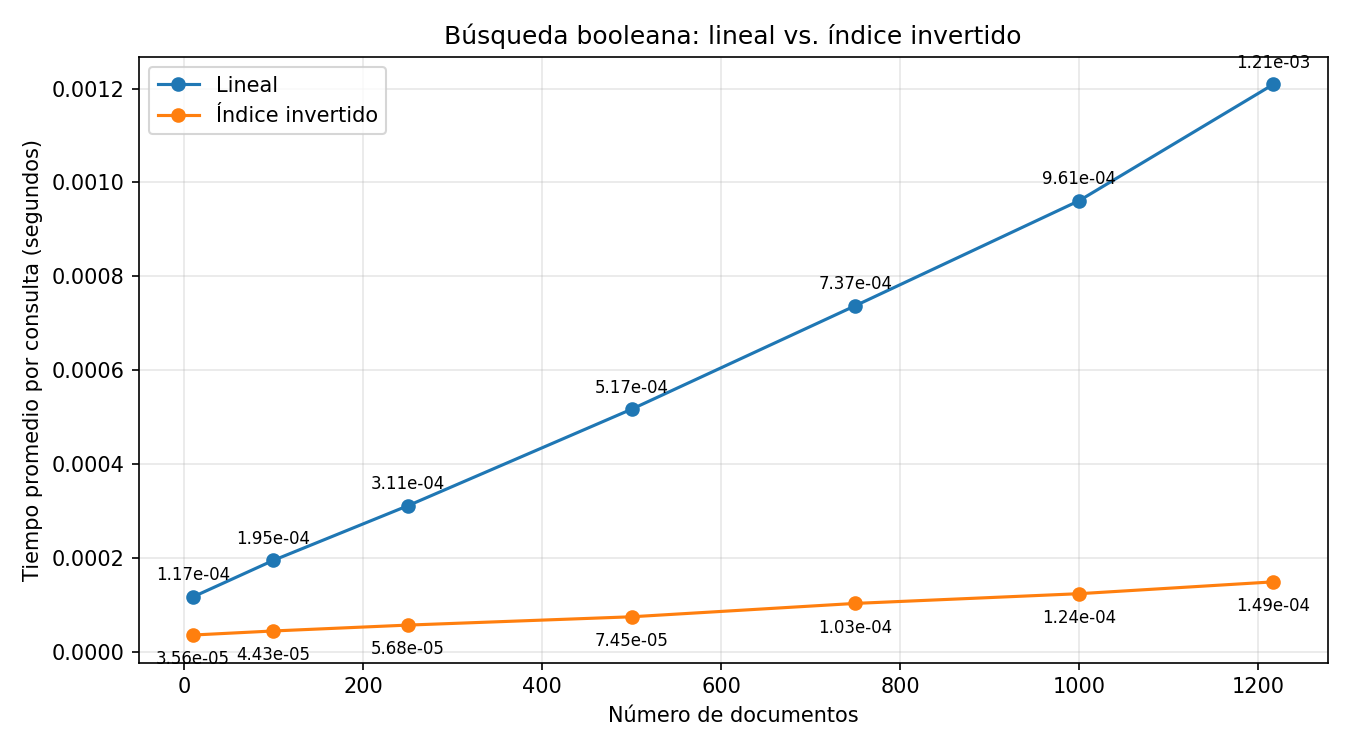
\includegraphics[width=0.88\linewidth]{resultados/booleana.png}
\caption{Búsqueda booleana: lineal vs.\ índice invertido.}
\end{figure}
\begin{figure}[H]\centering
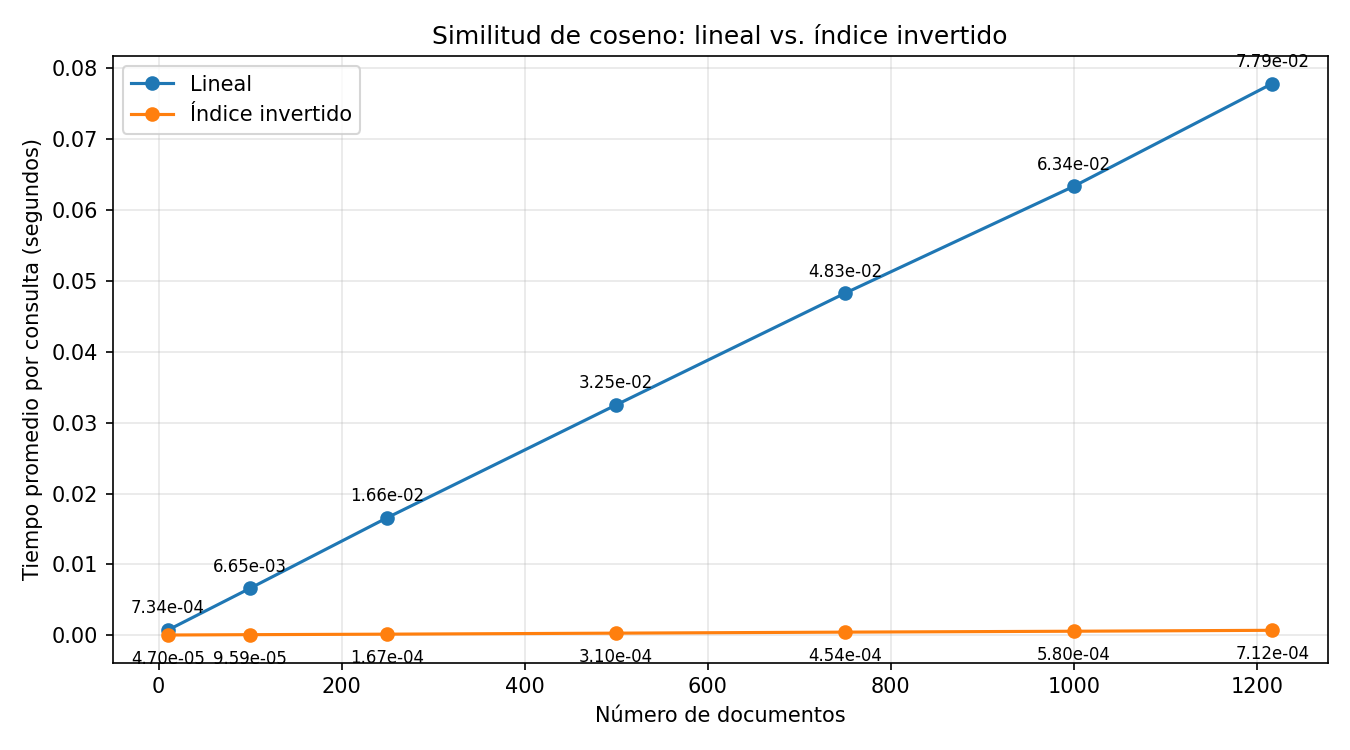
\includegraphics[width=0.88\linewidth]{resultados/coseno.png}
\caption{Similitud de coseno: lineal vs.\ índice invertido.}
\end{figure}

\section{P6. Análisis de resultados}
\textbf{1. Complejidad.} La booleana lineal es $O(N\cdot q)$, porque revisa el BoW de cada documento.
La booleana con índice es $O(\sum_{t\in q}|L(t)|)$, porque solo recorre las listas de los términos
consultados. El coseno lineal es $O(P)$, donde $P$ es el total de pares (término, documento), ya que en
cada consulta recalcula df, idf y normas. El coseno con índice es $O(\sum|L(t)| + C\log C)$, donde $C$
es el número de candidatos. Los datos lo confirman. De $N=10$ a $N=1217$ (122 veces más documentos),
el coseno lineal crece 106 veces (de 0.00073 s a 0.0779 s), casi proporcional a $N$. La booleana
lineal crece 10 veces (de 0.00012 s a 0.00121 s), porque con $N$ pequeño pesa el costo fijo de
analizar la consulta. Con índice el crecimiento es mucho menor: 4 veces en booleana y 15 en coseno.

\textbf{2. Punto de quiebre.} En tiempo de consulta, el índice gana desde el tamaño más pequeño medido
($N=10$) en ambos casos: 3.3 veces más rápido en booleana y 15.6 en coseno, así que los puntos
coinciden. Si se suma la construcción, ya no coinciden. En coseno, el índice se paga con unas 2
consultas. En booleana hacen falta entre 11 consultas ($N=10$) y 144 ($N=1217$).

\textbf{3. Overhead.} Sí: la construcción del índice. Toma 0.87 ms con $N=10$ y 152 ms con
$N=1217$, más que una búsqueda booleana lineal (0.12 ms y 1.21 ms). Ese tiempo se va en recorrer
todos los BoW, armar las listas y calcular idf y normas. Con pocas consultas booleanas, el índice no
conviene.

\textbf{4. Exactitud.} Las 9 consultas booleanas devolvieron los mismos IDs con ambos enfoques en los 7
tamaños. En coseno coinciden el top-5 y su orden. La diferencia máxima de score es $2.8\times10^{-17}$,
porque las sumas en coma flotante se hacen en distinto orden: el índice suma por término y el lineal
por documento. Los empates (por ejemplo, los documentos 96 y 143) se resuelven por id.

\textbf{5. Limitaciones.} Hoy el índice tiene 13\,330 términos y 180\,214 postings. Con 100 veces más
noticias tendría unos 18 millones de postings en tuplas de Python, es decir, varios GB de RAM. Además,
habría que reconstruirlo en cada ejecución, y eso pasaría de 0.15 s a decenas de segundos. La
alternativa es un índice persistente en disco: una tabla de PostgreSQL \code{(termino, doc\_id, tf)}
con índice B+Tree sobre \code{termino}, o un índice GIN sobre \code{tsvector}. Así solo se leen las
listas que la consulta necesita.

\end{document}
